\section{Einleitung}

  Spektroskopie, die Beobachtung von charakteristischen Wellenlängen von Licht welches Atome absorbiert und emittiert, ist eine der wichtigsten experimentellen Methoden. Mit einem dispersiven Element wird das Licht einer Quelle in seine verschiedenen Wellenlängen aufgespaltet. Die Position der Linien wird Spektrum genannt.

  Elektronen in einem Atom besetzen nur bestimmte Energieniveaus $E_i$; der Übergang von höheren Energieniveaus $E_2$ zu niedrigeren Energieniveaus $E_1$ führt zu einer Photonemission mit einer bestimmten Energie $E_{ph} = E_2 - E_1$, welche sich dann in Spektrum als Emmissionslinie beobachten lässt

  \subsection{Grundlagen des Zeeman-Effekts}
    Unter dem Zeeman-Effekt versteht man die Aufspaltung der atomaren Energieniveaus durch ein externes Magnetfeld. Um den Zeeman-Effekt in einer Näherung zu erklären betrachtet man ein Elektron, welches mit der Geschwindigkeit $\vec{v}$ im Abstand des Bohrradius $\vec{r}$ um den Atomkern bewegt und den Drehimpuls
    \begin{align}
    	\vec{l} = \vec{r} \times \vec{p} = m_e \cdot r \cdot v \cdot \vec{n}
    \end{align}
    aufweist. Des Weiteren kann das Elektron mit einem Strom
    \begin{align}
    	I = -e \cdot \frac{v}{2 \pi r}
    \end{align}
    und einem magnetischen Moment $\mu_l$
    \begin{align}
    	\vec{\mu_l} = I \cdot \vec{A} = I \cdot \pi r^2 \vec{n} = \frac{evr}{2}\vec{n}
    \end{align}
    beschrieben werden.

    Durch Interaktion eines externen Magnetfeldes mit dem magnetischen Moment ergibt sich eine Änderung der potentiellen Energie des Elektrons.
    \begin{align}
    	\Delta E_{pot} = - \vec{\mu_l} \cdot \vec{B} = \frac{e}{2m_e} \cdot \vec{l} \cdot \vec{B}
    \end{align}
    Mit Quantisierungsbedingungen bezüglich $\vec{l}$ und $\vec{B} \parallel \vec{l}$ vereinfacht sich die Gleichung zu
    \begin{align}
    	\Delta E_{pot} = \frac{e \cdot \hbar}{2m_e} \cdot m_l \cdot B = \mu_B \cdot m_l \cdot B
      \label{fml::3}
    \end{align}
    mit dem Bohr'schen Magneton $\mu_B$.

    Für Atome mit mehreren Elektronen kann man die $\vec{L} \vec{S}$-Kopplungsnäherung verwenden. Es werden aus Einzeldrehimpulsen ($\vec{L} = \sum_i \vec{l_i}$) und Einzelspins ($\vec{S} = \sum_i \vec{s_i}$) die Summen gebildet und daraus ein Gesamtdrehimpuls $\vec{J} = \vec{L} + \vec{S}$ erhalten. Daraus ergibt sich eine Energieänderung von
    \begin{align}
    	\Delta E_{pot} = \mu_B \cdot B \cdot M_J \cdot g_J
    \end{align}
    mit Landé-Faktor
    \begin{align}
    	g_J = 1 + \frac{J(J + 1) + S(S + 1) - L(L + 1)}{2J(J + 1)}
    \end{align}

    Ist $S = 0$ und $g_J = 1$ wird der Effekt \textbf{normaler} Zeeman-Effekt genannt, ansonsten \textbf{anomaler} Zeeman-Effekt.

  \subsection{Auswahlregeln}
    Nicht nur die Energie sondern auch Impuls-, Drehimpulserhaltung und Symmetrieeigenschaften spielen eine Rolle, ob überhaupt ein Übergang zwischen einem höheren Energieniveau $i$ zu einem niedrigeren Energieniveau $k$ stattfindet. Solche Übergänge sind nur möglich, wenn das Übergangsmatrixelement
    \begin{align}
    	\vec{M_{ik}} = e \int \Psi_i^* \; \vec{r} \; \Psi_k \; dV
    \end{align}
    mindestens eine Komponente ungleich Null besitzt.

    Dies ist dann der Fall, wenn gilt
    \begin{align*}
      \Delta M_J &= M_{J,i} - M_{J,k} = 0, \pm 1\\
      \Delta L &= \pm 1 \text{ und } \Delta S = 0
    \end{align*}
    Für $\Delta M_J = \pm 1$ ist ein zirkular polarisierendes Licht mit einer Phasenverschiebung von $\frac{\pi}{2}$ zu beobachten, der sogenannte $\sigma$-Übergang. Ein linear polarisierendes Licht ist für $\Delta M_J = 0$ zu beobachten, man spricht von einem $\pi$-Übergang.

  \subsection{Lummer-Gehrcke Platte}
    \begin{figure}[H]
    	\centering
    	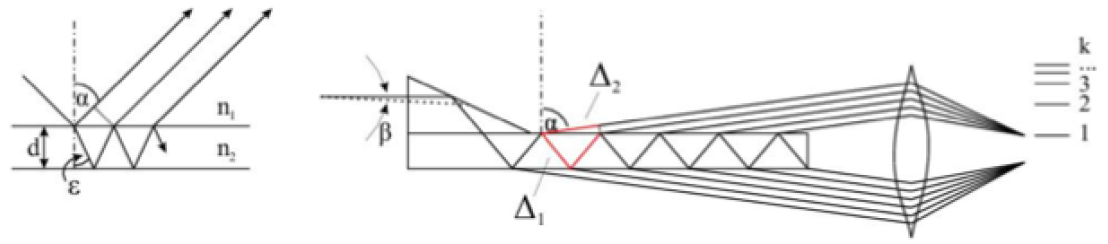
\includegraphics[scale=0.5]{parts/lummerGehrckePlate}
    	\caption{Lummer-Gehrcke Platte \cite{fp.booklet}}\label{fig:lummerGehrckePlatte}
    \end{figure}

    In diesem Versuch wird eine Lummer-Gehrcke Platte verwendet wodurch eine sehr hohe Auflösung erreicht wird, um den Effekt beobachten zu können. Die Platte besteht aus einer Quarzglasplatte mit extrem planparallelen Oberflächen. Das Licht wird durch ein Prisma in die Platte eingekoppelt und danach an den Innenseiten der planparallelen Platten unter einem Winkel nahe der Totalreflexion reflektiert. Die ausfallenden Lichtstrahlen interferieren miteinander und ermöglichen eine sehr hohe Auflösung. Der Gangunterschied ermittelt sich über
    \begin{align}
    	\Delta = 2n_2 \cdot \frac{d}{cos(\epsilon)} - 2n_1 \cdot d \cdot tan(\epsilon) \cdot sin(\alpha)
    \end{align}
    wobei $d$ die Dicke der Platte, $n_1$ und $n_2$ die Brechungsindizes außerhalb und innerhalb der Platte sind. Die Bezeichnungen $\alpha$ und $\epsilon$ sind aus \hyperref[fig:lummerGehrckePlatte]{Abb. \ref*{fig:lummerGehrckePlatte}} zu entnehmen.

    Aus geometrischen Relationen und der Näherung $n_2 \sim n$, $n_{air} = n_1 \sim 1$ und Austrittswinkel $\alpha \sim 90^\circ$ erhält man
    \begin{align}
    	\Delta = \Delta_1 - \Delta_2 = 2d \cdot \sqrt{n^2 - 1}
    \end{align}
    Für konstruktive Inteferenz muss der Gangunterschied $\Delta = k \cdot \lambda$, mit $k \in \mathbb{N} $ und der Wellenlänge $\lambda$, betragen.

    Den freien Spektralbereich der Lummer-Gehrcke Platte erhält man über
    \begin{align}
    	\Delta \lambda = \frac{\lambda^2}{2d \cdot \sqrt{n^2 - 1}}
      \label{fml::1}
    \end{align}
    Eine kleine Änderung in der Wellenlänge $\delta \lambda << \Delta \lambda$ führt zu einer Verschiebung
    \begin{align}
    	\delta \lambda = \frac{\delta a}{\Delta a} \cdot \Delta \lambda
    \end{align}
    wobei $\delta a$ die Distanz zwischen der Linie mit Wellenlänge $\lambda + \delta \lambda$ und der Position der Linie mit Wellenlänge $\lambda$; $\Delta a$ die Distanz zwischen den zwei Ordnungen $k$ und $k + 1$ der Wellenlänge $\lambda$.

  \subsection{Czerny-Turner Spektrometer}
    \begin{figure}[H]
    	\centering
    	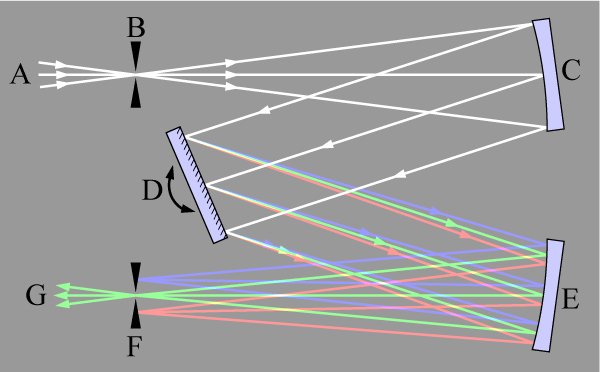
\includegraphics[scale=0.5]{parts/czernyTurnerSpectrometer_Wikipedia}
    	\caption{Czerny-Turner Spektrometer \cite{czerny.turner}}\label{fig:czernyTurnerSpectrometer}
    \end{figure}

    Licht, welches in das Spektrometer eintritt, wird zuerst mit Hilfe eines konkaven Spiegels parallelisiert. Danach trifft es auf ein Gitter und wird gebrochen. Das gebrochene Licht wird über einen weiteren konkaven Spiegel fokusiert und trifft anschließend auf eine CCD Kamera (siehe \hyperref[fig:czernyTurnerSpectrometer]{Abb. \ref*{fig:czernyTurnerSpectrometer}}).

    Die Dispersionseigenschaften eines Spektroskopieelements kann über eine Funktion $D(\lambda)$, bezogen auf wechselwirkende lineare Dispersion, beschrieben werden
    \begin{align}
    	D(\lambda) = \frac{\delta \lambda}{\delta p}
    \end{align}
    wobei $p$ die Position (bei der CCD Kamera in Pixel). Somit kann die Wellenlänge als Funktion der Position ermittelt werden
    \begin{align}
    	\lambda = \lambda_0 + \int_{p_0}^{p} D(\lambda) \; dp \label{lambdadispersion}
    \end{align}
    wobei $\lambda_0$ und $p_0$ bekannte Referenzpunkte sind. Ist die Dispersionsrelation unabhängig von $\lambda$ so kann \hyperref[lambdadispersion]{Gl. \eqref{lambdadispersion}} vereinfacht werden zu
    \begin{align}
    	\lambda = \lambda_0 + D(p - p_0)
    \end{align}

    \begin{figure}[H]
    	\centering
    	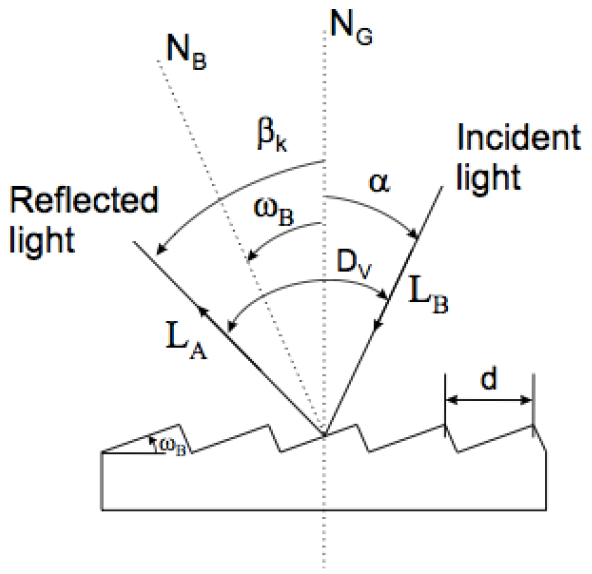
\includegraphics[scale=0.5]{parts/schematicReflectionGrating}
    	\caption{Schematische Darstellung einer Gitterreflexion \cite{fp.booklet}}\label{fig:schematicReflexionGrating}
    \end{figure}
